
%!TEX root = ../TTK4550-MHT.tex
\section{Survey of multi-target tracking methods}
\label{sec:survey}
The aim of this section is to give the reader a brief overview of tracking as a problem and a feeling for the most popular methods, their assumptions and strong and weak properties as seen from an two dimensional maritime anti collision perspective.

\subsection{Tracking}
Tracking of an object (target) is the process of estimating its state (i.e. position and velocity) based on discrete measurements from an observation system. An observation system can be a radar, sonar or any other sensor that passively or actively detects objects within an area or volume. Any observation system will be prone to noise, both in form of internal noise and external noise from the environment. This noise will, in varying degree, cause false measurements that the tracking system must take care of. These false measurements are often refereed to as clutter. 

\subsection{Tracking system}
A tracking system can be interpreted as either the complete system from the signal processing level to the finished tracks, or as I define it in this text: \emph{A system that process consecutive measurements from an observation system and collects measurements from the same target into tracks or initiate new tracks.} A track is a subset of all the measurements from the observation system that is believed to originate from the same target. The challenge knowing which measurement originating from which (real) target is the core at any tracking system. This association problem is non-trivial even under ideal situations, and the addition of spurious measurements and missed targets only increases the complexity.

There has been developed a large variety of methods to solve this association problem, and most of them have several sub-variants. In the following subsections, some of the most common and popular methods will be presented.

\subsection{Nearest Neighbour Filter}
\label{sec:nn}
The Nearest Neighbour Filter (NNF) is the simplest approach in tracking, where one always selects the closest neighbour as the consecutive measurement in the track, where the distance is the Euclidean distance (\ref{eq:euclidian_distance}).
\begin{equation}
D(z_k) = \left[ (z_k-z_{k-1}) \cdot (z_k-z_{k-1}) \right]^{1/2}
\label{eq:euclidian_distance}
\end{equation}
This approach suffers from being very vulnerable to clutter and dense target scenarios. It can be somewhat improved by estimating an a-priori state through a Kalman Filter and selecting the nearest neighbour to the estimate. This extension is sometimes refereed to as Nearest Neighbour Standard Filter (NNSF)\cite{Bar-Shalom1998} and also differs in that it used the Mahalanobis distance (\ref{eq:mahalanobis_distance}) which is a measure of the distance from a measurement to a distribution.
\begin{equation}
D(z_k) = \left[ z_k - \hat{z}_{k} \right]^T S(k+1)^{-1} \left[ z_k - \hat{z}_{k} \right]
\label{eq:mahalanobis_distance}
\end{equation}
Under the standard assumption that each target can at maximum generate one measurement, the NNF and NNSF are both single-target methods in the way that they may assign the same measurement to more that one track. They can, however, be expanded to multi-target variants by formulating the problem as a global least squares integer optimization problem, often called Global Nearest Neighbour Filter (GNNF). With this extension, the NNSF is almost becoming a zero-scan multi hypothesis tracker, in the sense that it seeks to select the optimal combination of mutual exclusive measurement-to-track associations while only looking at the most recent scan. NNF, NNSF and GNNF can be viewed as non-probabilistic models, as they do not assume specific models for noise, clutter, false alarm rate or similar.

\subsection{Probabilistic Data Association Filter}
\label{pdaf}
Probabilistic Data Association Filter (PDAF) is a \emph{single-target} Bayesian association filter which is based on single scan probabilistic analysis of measurements. The target is assumed initialized and modelled by (\ref{eq:kalman_model}). At each scan, the algorithm calculates the the association probabilities for all the measurement inside a validation gate, with the assumption that at most one of the measurements inside the validation gate is the true target. This leads to the state update equation (\ref{eq:pdaf_state_update}) where the current state is updated with a combined innovation.
\begin{equation}
\begin{split}
\V{\hat{y}}(k) &\triangleq \sum\limits_{j=1}^m \beta_j \V{ \tilde{y}_j } \\
\V{\hat{x}}(k|k) &= \V{\hat{x}}(k|k-1) + \M{K}(k) \V{\hat{y}}(k)
\end{split}
\label{eq:pdaf_state_update}
\end{equation} 
where
\begin{equation*}
\begin{split}
	\beta_j		&= \text{the probability of measurement j to be the correct one} \\
	\tilde{y}_j &= y_j - \hat{y}_j \hspace{5mm}	\text{the j-th measurement innovation} \\
	\M{K}(k) 	&= \text{the Kalman Gain for the k-th time step}
\end{split}
\end{equation*}
\begin{wrapfigure}[20]{R}{0.5\textwidth}
\centering
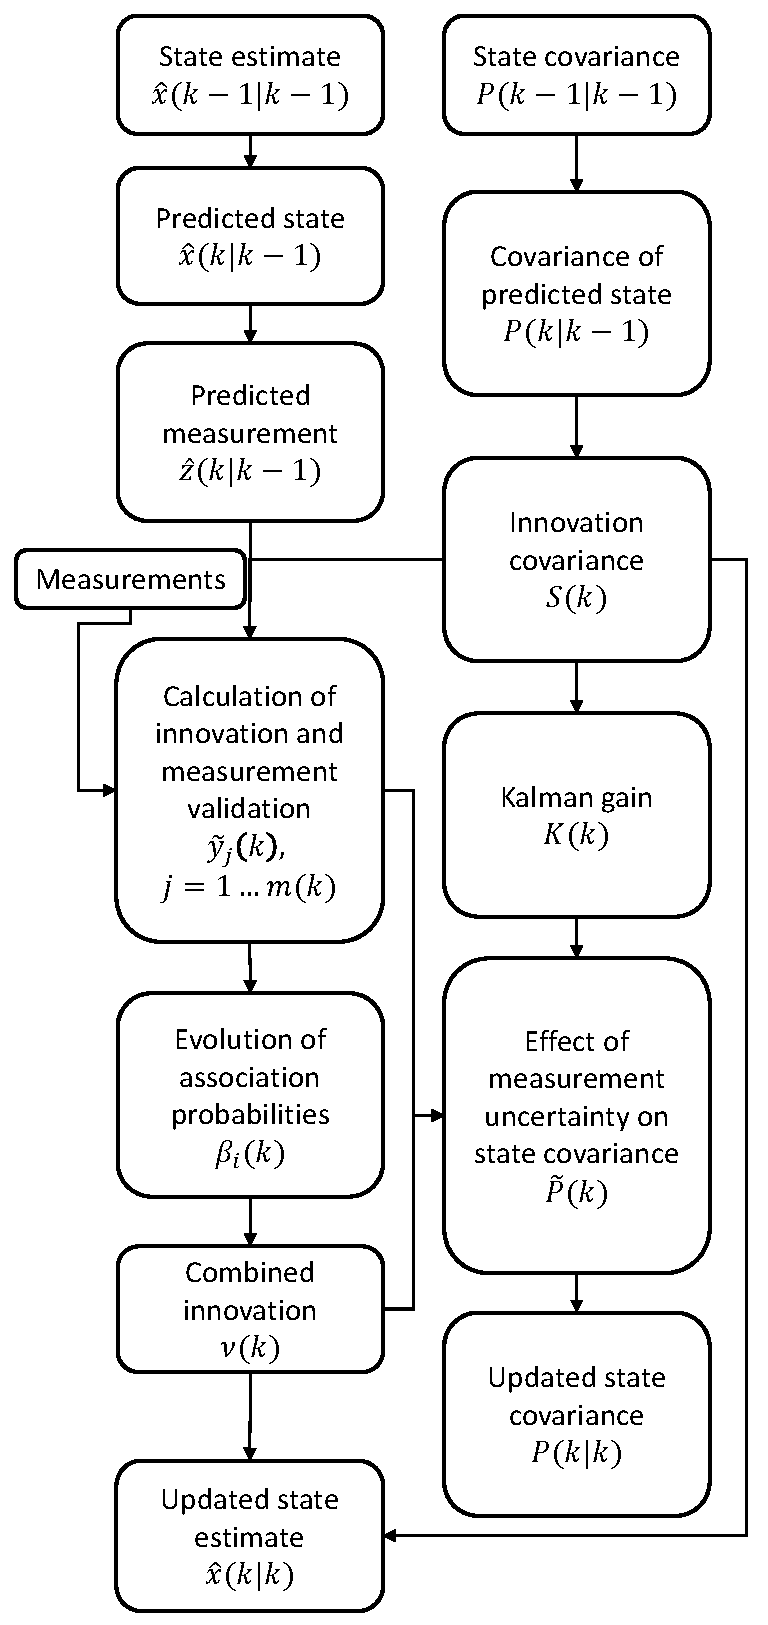
\includegraphics[height = .6\textheight]{pdaf-flowchart}
\caption{PDAF flowchart}
\label{fig:pdaf_flowchart}
\end{wrapfigure}
PDAF is computationally modest (approximate 50\% more computationally demanding than a Kalman Filter \cite{Bar-Shalom1998} p.163) and have good results in an environment with up to about 5 false measurement in a $4\sigma$ validation region \cite{Bar-Shalom1998}. PDAF does not include track initialization and assumes that at most one measurement can originate from an actual target. It also assumes that clutter is uniformly distributed in the measurement space and that the targets history is approximated by a Gaussian with a calculated mean and covariance.

PDAF can be used in multi target scenarios, but only as multiple copies of the single-target filter \cite{Fortmann1983}. PDAF can suffer from track coalescence, which is a phenomenon that merges two tracks into one. This coalescence occurs when two targets have similar paths, and the resulting tracks will be an "average" of the two (actual) tracks. There has been done some work to overcome this coalescence \cite{Blom2000}.



\subsection{Joint Probabilistic Data Association Filter}
\label{sec:jpdaf}
The Joint Probabilistic Data Association Filter (JPDAF) is a \emph{multi-target} extension of the Probabilistic Data Association Filter in which joint posteriori association probabilities are calculated for every target at each scan. Both PDAF and JPDAF use the same weighted sum (\ref{eq:pdaf_state_update}), the key difference is the way the weight $ \beta_j $ is calculated. Whereas PDAF treats all but one measurement inside its validation region as clutter, in JPDAF the targets which interacts (one cluster) are treated as connected and the connected $ \beta_j $s are computed jointly across the cluster set with a given set of active targets inside the cluster. The probability of a measurement $j$ belonging to a target
$ t $ is \cite{Fortmann1983}
\begin{equation}
\begin{split}
\beta_j^t &= \sum_{\chi} P\{ \chi | Y^k \} \hat{\omega}_{jt}(\chi) \\
\beta_0^t &= 1 - \sum_{j=1}^m \beta_j^t
\end{split}
\end{equation}
where
\begin{equation}
P\{\chi|Y^k\} = \frac{C^\phi}{c} 
				\prod_{j:\tau_j=1} \frac{exp[-\frac{1}{2}(\V{\tilde{y}_j^{t_j}})^T S_{t_j}^{-1}(\V{\tilde{y}^{t_j}})]}{(2\pi)^{M/2} |S_{t_j}|^{1/2}}
				\prod_{t:\delta_t=1} P_D^t
				\prod_{t:\delta_t=0} (1 - P_D^t).
\end{equation}
Where 
\begin{equation*}
\begin{split}
	\beta_j^k			&= \text{the probability that measurement j belongs to target k} \\
	\beta_0^k 			&= \text{the probability that no measurement belongs to target k} \\
	\chi 				&= \bigcap\limits_{j=1}^{m} \chi_{j t_j} \quad \text{All feasible events} \\
	Y^k 				&= \text{all candidate measurements up to and included time k} \\
	\hat{\omega}_{jt}	&=	\begin{cases}
								1, \text{if } \chi_{jt} \text{ occurs} \\ 
								0, \text{otherwise} 
							\end{cases} \\
	m					&= \text{number of measurements}
\end{split}
\end{equation*}
Since the JPDAF is calculating joint probabilities for all the combinations of measurement associations in the cluster, the computation demand is growing exponentially with the numbers of tracks and measurements in the cluster. A real time implementation of the JPDAF has been developed and patented by QinetiQ \cite{QinetiQ2003}, and described in \cite{Horridge}.

JPDAF also suffers from the same coalescence problem as the PDAF. Seen from a anti collision safety perspective is coalescence not acceptable. An improvement to the JPDAF has been proposed by \cite{Blom2000}.

Since JPDAF is using all the measurements inside the gate for each track, one measurement can be used to update more than one track if is within more that one gate.

\subsection{Multi Hypothesis Tracker}
\label{sec:mht}
Multiple hypothesis tracking (MHT) is a decision logic which generates and maintains alternative hypotheses when new measurement are received and within the gate. By making several possible hypotheses, the decision in which measurement to choose can be propagated into the future when more information is available. Each hypothesis is given a score or probability as a measure of the goodness of the measurement, which are accumulated to evaluate the combinations of consecutive measurements.

In contrast to PDA methods which in general will estimate an "average" of two closely spaced tracks as the true track (coalesce), MHT methods split when in doubt. The idea of using multiple hypotheses was first introduced by Singer. et al. \cite{Singer1974}, but the first complete algorithm was presented by Reid \cite{Reid1978}, where a hypothesis oriented MHT was developed. Following this, a track oriented MHT was proposed in \cite{Kurien1990} and the score function for MHT was later deduced and discussed by \cite{Bar-Shalom2007} since no explicit scoring function were given in \cite{Kurien1990}. MHT is, in the same way as PDAF/JPDAF, developed under the assumption that at most one measurement can originate from each target in each scan, and that a target does not necessary show on every scan (Probability of detection, $P_D < 1$).

Since MHT always selects the best tracks at any time, this can cause apparent inconsistency in the output to the user whenever a new set of measurements are received. If this is unwanted, an alternative representation is to output the N-best tracks and display them to the user in a way that visualises the probability. A third option is to output a weighted average of the tracks along with the covariance of the average.

The MHT approach to tracking and data association was by many for a long time dismissed because of its computationally large cost. The dramatic increase in computational capability from the 1980´s to the late 2010´s have however lead to a new spring for MHT with an increasing interest for use in tracking system. In 2004 Blackman stated \say{Multiple hypothesis tracking is generally accepted as the preferred method for solving the data association problem in modern multiple target tracking system}\cite{Blackman2004}. Already in 2001 did Blackman publish a demonstration that MHT is capable of real-time demands \cite{Blackman2001}.

There are two main approaches to MHT, hypothesis oriented and track oriented.

\subsubsection{Hypothesis Oriented MHT}
Hypothesis Oriented MHT (HOMHT) or Measurement Oriented MHT (MOMHT) is a tracking approach where direct probabilities of global joint measurement-to-target association hypothesis are calculated. The algorithm initiates tracks and handles missing measurements, it has a recursive nature and allows for clustering for quicker computation.

When a new set of measurements is received, Reid´s method defines a set of hypotheses, each containing a complete set of associations of the existing tracks and new measurements. By defining the hypotheses in this way, they become compatible in the sense that only one can and need to be selected. When the next set of measurements arrives, each of the current hypotheses are expanded with all measurement-to-track assignments for the new measurements. This way, the hypotheses will keep their compatibility.

When evaluating the alternative hypotheses, each is assigned a probability. This probability takes into account the false-alarm statistics of the measurement system, the expected density of targets and clutter and the accuracy of the target estimates. The probability of each data association hypothesis was developed by Reid in \cite{Reid1978}.
\begin{equation}
P_i^k = \frac{1}{c} P_D^{N_{DT}}(1-P_D)^{(N_{TGT}-N_{DT})} \beta_{FT}^{N_{FT}} \beta_{NT}^{N_{NT}} \left[ \prod_{m=1}^{N_{DT}} N(\V{Z_m}-\M{H}\V{\bar{x}},\M{B}) \right] P_g^{k-1}
\label{eq:homht_probability}
\end{equation}
where 
\begin{equation*}
\begin{split}
	P_i^k		&= \text{the probability of hypothesis $\Omega_i^k$ given measurements up through time $k$} \\
	P_D 		&= \text{the probability of detection} \\
	\beta_{FT} 	&= \text{the density of targets} \\ 
	\beta_{NT}	&= \text{the density of previously unknown targets that have been detected} \\
	N_{DT} 		&=	\text{number of designated target} \\
	N_{FT} 		&= \text{the number of false targets} \\
	N_{NT} 		&= \text{the number of new targets} \\
	N_{TGT} 	&= \text{is the number of targets} \\
	\V{Z_m} 	&= \text{the m-th measurement in the current scan} \\
	\M{H} 		&= \text{the observation matrix} \\
	\M{B} 		&= \text{the measurement covariance}
\end{split}
\end{equation*}

As with all MHT algorithms, it is crucial to prune the hypothesis tree to avoid an infinite memory and computational cost. In \cite{Reid1978}, several pruning techniques are used, it most important one is probably to remove all hypotheses with probability below a threshold. A second technique that were proposed is to merge hypotheses with the last N data scan in common. 

The initialization of tracks is done through the probabilities of each hypothesis, where a hypothesis would go from a tentative track to a confirmed track when the probability of that hypothesis exceeds i.e. $99 \%$. By treating all new measurement as tentative targets, and calculate their joint probability using information such as density of false targets, density of new targets and probability of detection and thresholding this, the algorithm has an advanced build-in initialization mechanism.

\subsubsection{Track Oriented MHT}
\label{subsec:tomht}
Track Oriented MHT (TOMHT) is a "bottom-up" approach where the tracks are assumed initialized, and for each scan the track splits whenever there are more than one feasible measurement in the validation region (in addition to the no-measurement hypothesis). This give rise to a track tree, as in Figure \ref{fig:hyp-tree}, where each initialized track has a root node and multiple branches, were each level represents a scan. A hypothesis is now a set of compatible tracks, with minimum and maximum one track from each track tree, were a hypothesis' score is the sum of its tracks score. Tracks are compatible if they do not share any measurements. The optimal hypothesis is the hypothesis with the highest score.

In the special case were each track tree does not share any measurements (single target), the optimal track is the leaf node with the highest score, which can be found by a traversal of the tree in logarithmic time. However, when a measurement is assigned to two or more targets, the problem of selecting the optimal combination of tracks becomes a multi dimensional assignment problem, since the best hypothesis from each track tree might be mutual exclusive.

New track hypotheses are generated from the filtered estimate from a Kalman Filter, and a score is calculated for instance using (20) from \cite{Bar-Shalom2007}. Both \cite{Bar-Shalom2007} and  \cite{Blackman2004} suggest that modern tracking system could improve performance in certain scenarios by using an Interacting Multiple Model (IMM) approach in stead of a single Kalman Filter. Following the addition of new track hypotheses, the tracks are divided into clusters, in which tracks with common measurements are grouped. The clusters can then be analysed as standalone global problems to find the best possible combination of (possibly mutual exclusive) measurement associations. Linear programming (LP)- and Integer Linear Programming (ILP)-based methods as proposed by \cite{Storms2003} can be used to find the best combinations of newly created track hypotheses in accordance to the assumption that a measurement only can be assigned to one target and that one target can maximally create one measurement.

To limit the size of the track hypothesis tree, various pruning schemes has been developed. The maybe single most important pruning is the N-scan pruning, also known as N-scan sliding window. This is a simple technique for limiting the size of the track tree and the following number of leaf nodes. The pruning is done by selecting the node that is N levels higher that the current best leaf node as new root node.

One of the largest drawback with the track oriented MHT approach is the lack of track initialization. This is because TOMHT only considers measurements that are within any (already initialized) targets gate, and automatically discards the unused measurements. The most common approach to add track initialization to TOMHT is to run a separate initialization algorithm in parallel with the tracking loop. This initialization method can be chosen freely, and some popular alternatives are; a dedicated HOMHT running on all or the unused measurements from the main loop, a N-of-M method that can be based on either nearest neighbour or PDA/JPDA or simply a manual initialization by the user. The options for this aiding module are endless, and the specific situation will influence the choice of method.